\documentclass[lualatex,ja=standard,a4paper,12pt]{bxjsarticle}
\usepackage{amsmath, amssymb, amsthm}
\usepackage{geometry}
\usepackage{xcolor}
\usepackage{tcolorbox}
\usepackage{booktabs}
\usepackage{array}
\usepackage{graphicx}
\usepackage{listings}
\usepackage{tikz}
\usetikzlibrary{arrows.meta, positioning}

\geometry{margin=25mm}

\tcbuselibrary{theorems, skins, breakable}

\newtcolorbox{defbox}[1]{
  colback=blue!5, colframe=blue!60!black,
  fonttitle=\bfseries, title={#1}, arc=3pt, breakable
}
\newtcolorbox{thmbox}[1]{
  colback=green!5, colframe=green!50!black,
  fonttitle=\bfseries, title={#1}, arc=3pt, breakable
}
\newtcolorbox{pointbox}{
  colback=orange!8, colframe=orange!70!black,
  fonttitle=\bfseries, title={ポイント}, arc=3pt, breakable
}
\newtcolorbox{exbox}[1]{
  colback=gray!6, colframe=gray!50,
  fonttitle=\bfseries, title={例：#1}, arc=3pt, breakable
}
\newtcolorbox{warningbox}{
  colback=red!5, colframe=red!60!black,
  fonttitle=\bfseries, title={注意}, arc=3pt, breakable
}

\lstset{
  basicstyle=\ttfamily\small,
  frame=single,
  framesep=6pt,
  rulecolor=\color{gray!50},
  backgroundcolor=\color{gray!4},
  breaklines=true,
  showstringspaces=false,
  columns=flexible,
}

\title{{\large Hoff 第6章} \\[6pt]
       \textbf{6.4\; Gibbs Sampling} \\[4pt]
       {\normalsize （ギブスサンプリング）ゼミ資料}}
\author{}
\date{}

\begin{document}
\maketitle
\thispagestyle{empty}

% ===========================
\section{6.3節の宿題}
% ===========================

6.3節で，2つの完全条件付き分布
\[
  p(\theta \mid \sigma^2, \boldsymbol{y}) = \mathrm{Normal}(\mu_n, \tau_n^2),
  \qquad
  p(\sigma^2 \mid \theta, \boldsymbol{y}) = \mathrm{inverse\text{-}gamma}\!\left(\tfrac{\nu_n}{2}, \tfrac{\nu_n\sigma_n^2(\theta)}{2}\right)
\]
を交互に使えば同時事後分布からの標本が作れる，という見通しが立った．
ただし議論は\textbf{出発点 $\sigma^{2(1)}$ を周辺分布から引けること}を仮定しており，
そこが循環していた．

\medskip
本節での答えは身も蓋もない：
\begin{center}
\textbf{出発点は適当に決めてよい．そのまま繰り返せばよい．}
\end{center}

\noindent これを手続きとして定義したものが\textbf{ギブスサンプラー}である．

% ===========================
\section{ギブスサンプラーの定義}
% ===========================

\begin{defbox}{完全条件付き分布（full conditional distribution）}
$p(\theta \mid \sigma^2, y_1, \ldots, y_n)$ と
$p(\sigma^2 \mid \theta, y_1, \ldots, y_n)$ を，それぞれ
$\theta$ と $\sigma^2$ の\textbf{完全条件付き分布}と呼ぶ．
「完全」とは，\textbf{そのパラメータ以外のすべて}を条件にしている，という意味である．
\end{defbox}

\begin{defbox}{ギブスサンプラー（Gibbs sampler）}
パラメータの現在の状態を
$\phi^{(s)} = \{\theta^{(s)}, \tilde{\sigma}^{2(s)}\}$ とする．
次の状態を以下の手順で生成する：
\begin{enumerate}
  \item $\theta^{(s+1)} \sim p(\theta \mid \tilde{\sigma}^{2(s)}, y_1, \ldots, y_n)$ を引く
  \item $\tilde{\sigma}^{2(s+1)} \sim p(\tilde{\sigma}^2 \mid \theta^{(s+1)}, y_1, \ldots, y_n)$ を引く
  \item $\phi^{(s+1)} = \{\theta^{(s+1)}, \tilde{\sigma}^{2(s+1)}\}$ とおく
\end{enumerate}
これを繰り返して得られる列
$\{\phi^{(1)}, \phi^{(2)}, \ldots, \phi^{(S)}\}$ を
ギブスサンプラーの出力とする．
\end{defbox}

\begin{pointbox}
\textbf{手順2で $\tilde{\sigma}^{2(s)}$ ではなく $\theta^{(s+1)}$ を使うこと}

$\sigma^2$ を更新するときに条件とするのは，
\textbf{いま引いたばかりの}$\theta^{(s+1)}$ であって，
1つ前の $\theta^{(s)}$ ではない．
6.3節の連鎖の議論がまさにこの形（引いた値をただちに次の条件にする）
だったことを思い出したい．
\end{pointbox}

\begin{warningbox}
\textbf{得られる列は独立ではない}

Hoff は \textit{``generates a \textbf{dependent} sequence of our parameters''}
と明記している．
$\phi^{(s+1)}$ は $\phi^{(s)}$ を使って作られるので，隣り合う標本は相関する．

\medskip
第4章までの\textbf{独立な}モンテカルロ標本とはここが決定的に違う．
標本平均が事後平均に近づくこと自体は成り立つが，
「標本の数 $S$ 個ぶんの情報がある」とは言えなくなる．
どれだけ情報が目減りするかを測るのが6.6節の話題（自己相関・有効標本サイズ）である．
\end{warningbox}

\paragraph{6.3節との違いは一点だけ}
6.3節の議論は「$\sigma^{2(1)}$ が\textbf{周辺事後分布からの標本}であるとき」
という条件付きだった．
ギブスサンプラーはその要求を\textbf{単に取り下げる}．
出発点はどこでもよいことにして，あとは同じ操作を繰り返す．

\medskip
これで「正しい出発点が要る」という循環は消えるが，代わりに
\textbf{「適当な出発点から始めて本当に正しい分布に行き着くのか」}
という問題が生じる．
本節ではそれを\textbf{実例で確かめる}にとどめ，
理論的な保証は6.6節に委ねる．

% ===========================
\section{R による実装}
% ===========================

\begin{lstlisting}[language=R]
### data
mean.y <- mean(y) ; var.y <- var(y) ; n <- length(y)

### starting values
S <- 1000
PHI <- matrix(nrow = S, ncol = 2)
PHI[1,] <- phi <- c(mean.y, 1/var.y)

### Gibbs sampling
set.seed(1)
for(s in 2:S) {

  # generate a new theta value from its full conditional
  mun  <- (mu0/t20 + n*mean.y*phi[2]) / (1/t20 + n*phi[2])
  t2n  <- 1/(1/t20 + n*phi[2])
  phi[1] <- rnorm(1, mun, sqrt(t2n))

  # generate a new 1/sigma^2 value from its full conditional
  nun  <- nu0 + n
  s2n  <- (nu0*s20 + (n-1)*var.y + n*(mean.y - phi[1])^2) / nun
  phi[2] <- rgamma(1, nun/2, nun*s2n/2)

  PHI[s,] <- phi
}
\end{lstlisting}

\paragraph{出発点}
\texttt{phi <- c(mean.y, 1/var.y)}，すなわち
$\theta^{(1)} = \bar{y}$，$\tilde{\sigma}^{2(1)} = 1/s^2$ である．
事後分布からの標本などではなく，\textbf{ただの標本統計量}を置いているだけ
——「適当に決めてよい」を実際にやっている．

\paragraph{\texttt{phi[1]} の更新直後に \texttt{phi[1]} を使っている}
3行目で \texttt{phi[1]} を上書きし，その下の \texttt{s2n} の計算で
その新しい \texttt{phi[1]} を参照している．
これが定義の手順2（$\theta^{(s+1)}$ で条件付ける）に対応している．

\paragraph{使っている恒等式}
コード中の \texttt{s2n} は，定義の
$\sigma_n^2(\theta) = [\nu_0\sigma_0^2 + n s_n^2(\theta)]/\nu_n$ を，
次の平方和の分解で書き換えたものである：
\begin{align*}
  n s_n^2(\theta) = \sum_{i=1}^{n}(y_i - \theta)^2
  &= \sum_{i=1}^{n}(y_i - \bar{y} + \bar{y} - \theta)^2 \\
  &= \sum_{i=1}^{n}\left[(y_i - \bar{y})^2 + 2(y_i - \bar{y})(\bar{y} - \theta) + (\bar{y} - \theta)^2\right] \\
  &= \sum_{i=1}^{n}(y_i - \bar{y})^2 + \underbrace{2(\bar{y}-\theta)\sum_{i=1}^{n}(y_i - \bar{y})}_{=\,0} + \sum_{i=1}^{n}(\bar{y} - \theta)^2 \\
  &= (n-1)s^2 + n(\bar{y} - \theta)^2.
\end{align*}
交差項が消えるのは $\sum (y_i - \bar{y}) = 0$ だからである．

\begin{pointbox}
\textbf{なぜわざわざこう書くのか}

$\bar{y}$ と $s^2$ は\textbf{反復のたびに変わらない}（データだけで決まる）ので，
ループの外で一度計算しておけばよい．
反復の中で必要なのは $n(\bar{y}-\theta)^2$ という\textbf{スカラーの計算1回}だけになる．
素直に $\sum_{i=1}^{n}(y_i - \theta)^2$ を毎回計算すると
$n$ 個の引き算と二乗が毎反復で発生する．

\medskip
$n = 9$ では差は出ないが，$n$ が大きく $S$ が数万回になると効いてくる．
「十分統計量をループの外に出す」のは MCMC 実装の定石である．
\end{pointbox}

% ===========================
\section{実行結果}
% ===========================

ユスリカのデータと6.2節と同じ事前分布のもとで，1000反復のギブスサンプラーを走らせる．

\subsection*{軌跡を見る}

\begin{figure}[htbp]
\centering
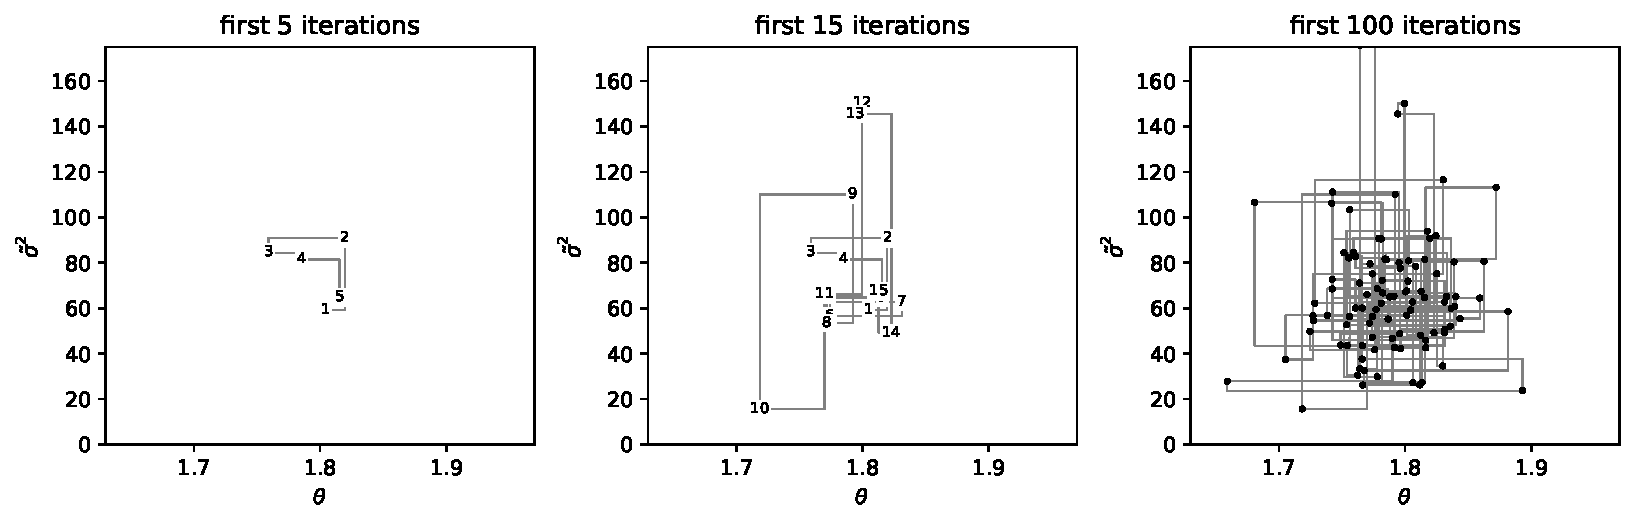
\includegraphics[width=\textwidth]{fig6_2.pdf}
\caption{ギブスサンプラーの最初の5，15，100反復．
番号は反復の順番．Hoff の Figure 6.2 に対応．
各状態を結ぶ線が\textbf{階段状}になっているのは，
$\theta$ の更新が横移動，$\tilde{\sigma}^2$ の更新が縦移動だからである．}
\end{figure}

\noindent 動きの特徴：
\begin{itemize}
  \item 1反復で\textbf{横→縦}と直角に動く．
        2つのパラメータを\textbf{同時にではなく交互に}更新しているため．
  \item 最初の数回で，出発点 $(\bar{y}, 1/s^2) = (1.804,\ 59.4)$ の周辺から
        事後分布の広がり全体へ散っていく．
  \item 100反復も回すと，点が事後分布の形をなぞるように溜まっていく．
\end{itemize}

\subsection*{1000標本と事後分布}

\begin{figure}[htbp]
\centering
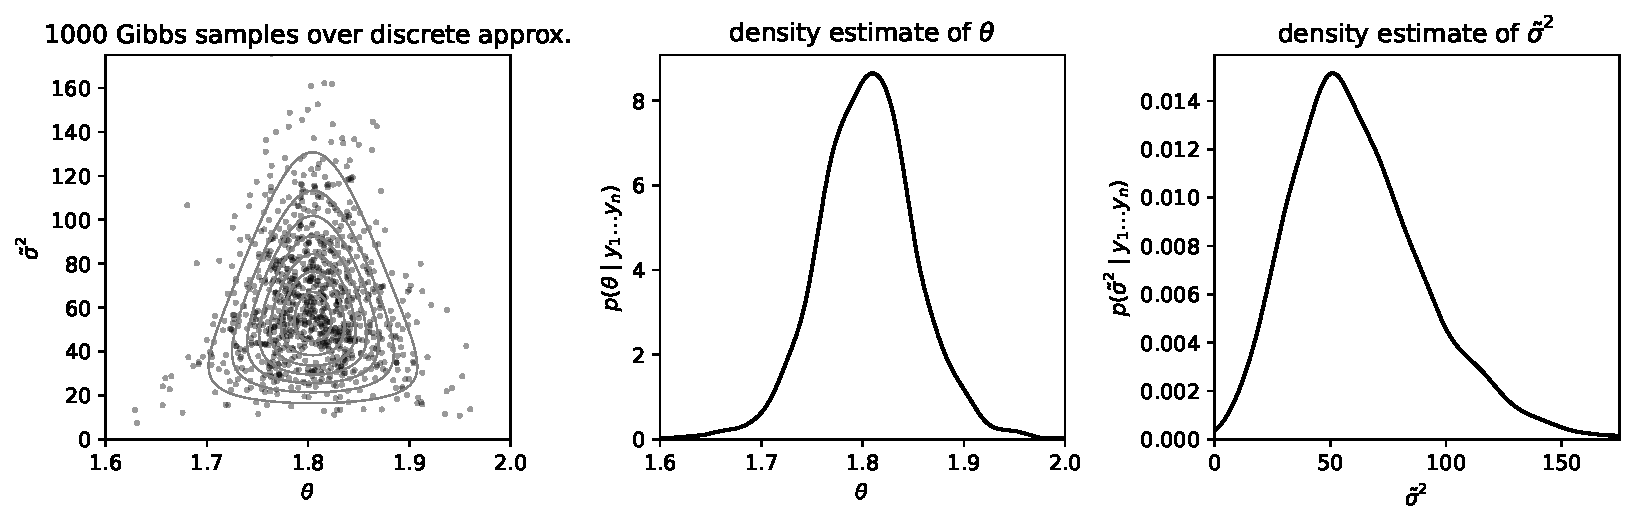
\includegraphics[width=\textwidth]{fig6_3.pdf}
\caption{左：1000個のギブス標本を，6.2節の離散近似の等高線に重ねたもの．
中・右：標本から推定した $\theta$ と $\tilde{\sigma}^2$ の周辺事後密度．
Hoff の Figure 6.3 に対応．}
\end{figure}

\begin{pointbox}
\textbf{この例の意義：答え合わせができる}

6.2節の離散近似（図6.1）と，本節のギブス標本（図6.3）は，
\textbf{同じ事後分布を別々の方法で求めたもの}である．
2つがほぼ重なるという事実が，
ギブスサンプラーが正しく動いていることの\textbf{証拠}になる．

\medskip
もっとも，この2パラメータの問題ではそもそもギブスサンプラーは\textbf{必要ない}
——離散近似で十分だからである．
ギブスサンプラーが本当に必要なのは離散近似が使えない高次元の問題であり，
そこでは\textbf{この答え合わせができない}．
だからこそ，手法の正しさを理論的に保証することと，
収束を診断する道具を持つこと（6.6節）が重要になる．
\end{pointbox}

\subsection*{事後分位点}

標本が手に入れば，事後区間は\texttt{quantile()}を呼ぶだけである．

\begin{lstlisting}[language=R]
### CI for population mean
> quantile(PHI[,1], c(.025, .5, .975))
    2.5%      50%     97.5%
1.707282 1.804348  1.901129

### CI for population precision
> quantile(PHI[,2], c(.025, .5, .975))
    2.5%      50%     97.5%
17.48020 53.62511 129.20020

### CI for population standard deviation
> quantile(1/sqrt(PHI[,2]), c(.025, .5, .975))
      2.5%        50%      97.5%
0.08797701 0.13655763 0.23918408
\end{lstlisting}

\begin{center}
\renewcommand{\arraystretch}{1.4}
\begin{tabular}{llrrr}
\toprule
 & & 2.5\% & 50\% & 97.5\% \\
\midrule
母平均 $\theta$ & Hoff（R） & 1.707 & 1.804 & 1.901 \\
                & 再現（Python） & 1.708 & 1.805 & 1.900 \\
\midrule
母精度 $\tilde{\sigma}^2$ & Hoff（R） & 17.48 & 53.63 & 129.20 \\
                & 再現（Python） & 16.89 & 58.02 & 129.18 \\
\midrule
母標準偏差 $\sigma$ & Hoff（R） & 0.0880 & 0.1366 & 0.2392 \\
                & 再現（Python） & 0.0880 & 0.1313 & 0.2433 \\
\bottomrule
\end{tabular}
\end{center}

\noindent 乱数の種・生成器が違うので完全一致はしないが，よく一致している．
一致の精度（たとえば $\tilde{\sigma}^2$ の中央値が 53.6 対 58.0）が
\textbf{この手法の誤差の目安}でもある．

\begin{pointbox}
\textbf{標準偏差の区間が「変換するだけ」で出ること}

3つ目の \texttt{quantile(1/sqrt(PHI[,2]), ...)} に注目したい．
$\tilde{\sigma}^2$ の標本を $1/\sqrt{\tilde{\sigma}^2} = \sigma$ に
\textbf{1つずつ変換して分位点を取っただけ}である．
$\sigma$ の事後分布を解析的に求める必要も，
ヤコビアンを考える必要もない．

\medskip
これは標本に基づく方法の一般的な強みで，
$\theta/\sigma$ でも $\Pr(\theta > 1.8 \mid \boldsymbol{y})$ でも，
\textbf{パラメータの任意の関数}の事後分布が同じやり方で得られる．
\end{pointbox}

% ===========================
\section{何が解決して，何が残ったか}
% ===========================

\begin{thmbox}{6.4節のまとめ}
\begin{enumerate}
  \item \textbf{ギブスサンプラー}は，完全条件付き分布から
        $\theta \to \sigma^2 \to \theta \to \cdots$ と交互に引くだけの手続きである．
        6.3節の循環は「出発点は適当でよい」と\textbf{要求を取り下げる}ことで断ち切った．

  \item 実装上は，平方和の分解
        $\sum(y_i-\theta)^2 = (n-1)s^2 + n(\bar{y}-\theta)^2$ を使って
        $\bar{y}$ と $s^2$ をループの外に出す．

  \item ユスリカのデータで1000反復回すと，得られた標本の分布は
        6.2節の離散近似と\textbf{ほぼ一致}した．
        標本さえあれば，$\sigma$ のような変換後の量の事後区間も変換するだけで得られる．
\end{enumerate}
\end{thmbox}

\begin{warningbox}
\textbf{残っている問題}

\begin{enumerate}
  \item \textbf{正しさは証明されていない．}
        Hoff の書き方も
        \textit{``This gives some \underline{indication} that the Gibbs sampling
        procedure is a valid method''}（妥当であることの\textbf{示唆}を与える）
        であって，証明ではない．
        一般的な保証は6.5節・6.6節で与えられる．

  \item \textbf{標本が独立でない．}
        隣り合う標本は相関するので，
        $S = 1000$ 個あっても独立な1000標本ぶんの情報はない．

  \item \textbf{出発点の影響がいつ消えるか分からない．}
        図6.2の最初の数反復は明らかに出発点の近くにいる．
        実務では初期の一定回数を捨てる（burn-in）が，
        何回捨てればよいかは自明でない．
\end{enumerate}

\noindent これら3つが，6.5節（一般的な性質）と6.6節（MCMC診断）の主題になる．
\end{warningbox}

\end{document}
